\section{DMD-LSTM Model Results and Discussions}
\label{sec:dmd_res}
This section presents and discusses the Deep Learning Model's 
training, testing, and cross-validation results.

In Table \ref{tab:dmd_lstm_training_scores} the training error metrics
are shown for each of the window sizes tested. \\
% tab:dmd_lstm_training_scores
\begin{longtable}[c]{ccccc}
    \caption{DMD-LSTM Training Error Metrics Scores for Different Window Sizes}
    \label{tab:dmd_lstm_training_scores}\\
    \hline
                                             & \multicolumn{4}{c}{\textit{Window Sizes}}                                          \\
    \multirow{-2}{*}{\textbf{Error Metrics}} & \textbf{5}                               & \textbf{10} & \textbf{15} & \textbf{20} \\ \hline
    \endfirsthead
    %
    \multicolumn{5}{c}%
    {{\bfseries Table \thetable\ continued from previous page}} \\
    \hline
                                             & \multicolumn{4}{c}{\textit{Window Sizes}}                                          \\
    \multirow{-2}{*}{\textbf{Error Metrics}} & \textbf{5}                               & \textbf{10} & \textbf{15} & \textbf{20} \\ \hline
    \endhead
    %
    \hline
    \endfoot
    %
    \endlastfoot
    %
    \textbf{MSE}                             & 0.000037                                 & 0.787877    & 0.006917    & 0.057851    \\
    \textbf{RMSE}                            & 0.006106                                 & 0.887624    & 0.083166    & 0.240522    \\
    \textbf{MAE}                             & 0.004175                                 & 0.755407    & 0.067645    & 0.202746    \\
    \textbf{MAPE}                            & {\color[HTML]{32CB00} \textbf{0.000001}} & 0.000194    & 0.000017    & 0.000053    \\ \hline
\end{longtable}}
Where it is observed that the best performing model based on
having the lowest MAPE score is the DMD-LSTM with a window
size of 5. Morever, we can see the differences from each
MAPE score for each window size in the Figure 
\ref{fig:dmd_lstm_training_MAPE} shown below. \\
\begin{figure}[ht]
    \centering
    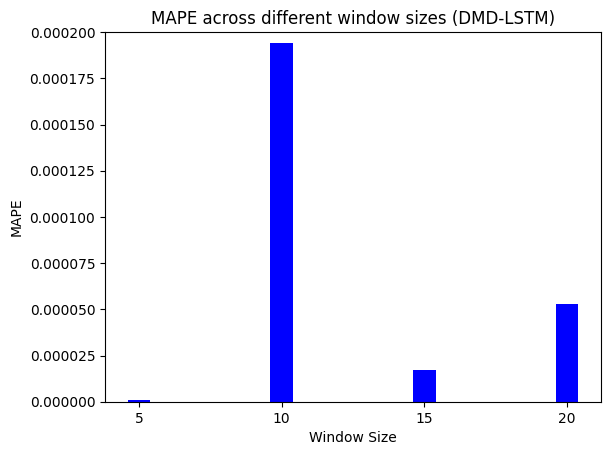
\includegraphics[width=1\textwidth]{./assets/Chapter_4/DMD_LSTM_Training/DMD_LSTM_MAPE.png}
    \caption{Comparison of MAPE Scores for DMD-LSTM Model Training Across Different Window Sizes}
    \label{fig:dmd_lstm_training_MAPE}
\end{figure}
\FloatBarrier
The figure above also shows that the MAPE score for window sizes 15 
and 20 is higher than the MAPE score for window size 10. MAPE score 
increases from window size 15 to size 20, indicating that increasing 
window size may result in a lower performing model.
\\

Furthermore, as previously stated, the window size of 5 results in 
the best MAPE score being the lowest. Where it outperforms the worst 
performing model (DMD-LSTM with window size 10) by 0.000193 units. 
As illustrated clearly in Figure \ref{fig:dmd_lstm_training_MAPE}.
\\

Knowing that the DMD-LSTM model performs as expected based on the 
training data scores, it is critical that we also examine the 
training data results from a baseline LSTM. The baseline LSTM is, 
as the name implies, a simple LSTM model lacking the DMD component. 
The table below shows the results of the baseline LSTM training.
\\

% tab:baseline_lstm_training
\begin{longtable}[c]{ccccc}
    \caption{Baseline LSTM Training Error Metrics Scores for Different Window Sizes}
    \label{tab:baseline_lstm_training}\\
    \hline
                                             & \multicolumn{4}{c}{\textit{Window Sizes}}                                                              \\
    \multirow{-2}{*}{\textbf{Error Metrics}} & \textbf{5}                      & \textbf{10}                              & \textbf{15} & \textbf{20} \\ \hline
    \endfirsthead
    %
    \multicolumn{5}{c}%
    {{\bfseries Table \thetable\ continued from previous page}} \\
    \hline
                                             & \multicolumn{4}{c}{\textit{Window Sizes}}                                                              \\
    \multirow{-2}{*}{\textbf{Error Metrics}} & \textbf{5}                      & \textbf{10}                              & \textbf{15} & \textbf{20} \\ \hline
    \endhead
    %
    \hline
    \endfoot
    %
    \endlastfoot
    %
    \textbf{MSE}                             & 2912.840703                     & 191.935882                               & 1118.183283 & 706.136814  \\
    \textbf{RMSE}                            & 53.970739                       & 13.854093                                & 33.439248   & 26.573235   \\
    \textbf{MAE}                             & 35.301888                       & 9.480864                                 & 22.099720   & 18.285352   \\
    \textbf{MAPE}                            & {\color[HTML]{333333} 0.009618} & {\color[HTML]{32CB00} \textbf{0.002527}} & 0.006024    & 0.005004    \\ \hline
\end{longtable}}
According to the table above, the baseline LSTM with window size 
10 performs the best, with the lowest MAPE score of 0.002527 
when compared to the other baseline LSTM models.
\\

However, the DMD-LSTM model with window size 5 outperforms it by 
0.002526. 
As a result, the alamSYS makes use of the DMD-LSTM model, 
specifically the one with a window size of 5. 
Where from now on, the DMD-LSTM model refers to 
the DMD-LSTM model with a window size of 5.
\\

Nonetheless, the DMD-LSTM model's performance is limited to the 
training dataset from PSEI, and it must be cross-validated using 
data from other stocks, which includes the PSEI validation dataset.
The results of this cross-validation is presented in Table
\ref{tab:dmd-lstm_cross}. It should also be noted that 
cross-validation uses logarithmic normalization as a data 
preprocessing technique to make the dataset more normal, 
which aids in analyzing the model's performance with the given 
dataset. Normalization techniques, in particular, allow for closer 
variation within the forecasted data.
\cite{Patro2015}.

% tab:dmd-lstm_cross
\begin{longtable}[c]{ccccc}
    \caption{DMD-LSTM Cross-Validation Error Metrics Scores}
    \label{tab:dmd-lstm_cross}\\ \hline
    \textbf{Stocks} & \textbf{MSE}                   & \textbf{RMSE} & \textbf{MAE} & \textbf{MAPE}                       \\
    \hline
    \endfirsthead
    %
    \multicolumn{5}{c}%
    {{\bfseries Table \thetable\ continued from previous page}} \\ \hline
    \textbf{Stocks} & \textbf{MSE}                   & \textbf{RMSE} & \textbf{MAE} & \textbf{MAPE}                       \\
    \hline
    \endhead
    %
    \textbf{PSEI}   & 0.00002                        & 0.00419       & 0.00328      & 1.510000e-03                        \\
    \textbf{AC}     & 0.00236                        & 0.04856       & 0.03414      & 6.110000e-03                        \\
    \textbf{ALI}    & 0.00255                        & 0.05054       & 0.03645      & 1.597000e-02                        \\
    \textbf{AP}     & 0.00129                        & 0.03596       & 0.02515      & 9.220000e-03                        \\
    \textbf{BDO}    & 0.00160                        & 0.03999       & 0.02799      & 7.250000e-03                        \\
    \textbf{BLOOM}  & 0.01883                        & 0.13721       & 0.06901      & {\color[HTML]{FE0000} 1.052898e+12} \\
    \textbf{FGEN}   & 0.00224                        & 0.04733       & 0.03265      & 1.197000e-02                        \\
    \textbf{GLO}    & 0.00211                        & 0.04595       & 0.03149      & 4.680000e-03                        \\
    \textbf{ICT}    & 0.00335                        & 0.05785       & 0.03731      & {\color[HTML]{FE0000} 3.005818e+11} \\
    \textbf{JGS}    & 0.00331                        & 0.05752       & 0.03992      & {\color[HTML]{FE0000} 2.009923e+11} \\
    \textbf{LTG}    & 0.01567                        & 0.12518       & 0.05858      & {\color[HTML]{FE0000} 3.583335e+12} \\
    \textbf{MEG}    & 0.00431                        & 0.06565       & 0.04422      & {\color[HTML]{FE0000} 1.393042e+11} \\
    \textbf{MER}    & 0.00326                        & 0.05708       & 0.03770      & 9.170000e-03                        \\
    \textbf{MPI}    & 0.00273                        & 0.05230       & 0.03390      & 2.497000e-02                        \\
    \textbf{PGOLD}  & 0.00149                        & 0.03865       & 0.02818      & 7.880000e-03                        \\
    \textbf{RLC}    & 0.00338                        & 0.05817       & 0.03978      & 6.922000e-02                        \\
    \textbf{RRHI}   & 0.00131                        & 0.03618       & 0.02699      & 6.390000e-03                        \\
    \textbf{SMC}    & 0.00137                        & 0.03702       & 0.02317      & 5.690000e-03                        \\
    \textbf{TEL}    & 0.00178                        & 0.04214       & 0.03002      & 4.240000e-03                        \\
    \textbf{URC}    & 0.00297                        & 0.05447       & 0.03742      & 1.798000e-02                        \\ \hline
\end{longtable}}
As shown in the table above, the chosen DMD-LSTM model performs well 
across all other stocks, demonstrating that the model is not 
overfitted to the training dataset. This score additionally suggests 
that the model works with non-training data.
\\

The figures below show a 100-day worth of predicted prices versus 
actual prices to better visualize the performance of the DMD-LSTM 
model for each stock.
\\

% AC
\begin{figure}[ht]
    \centering
    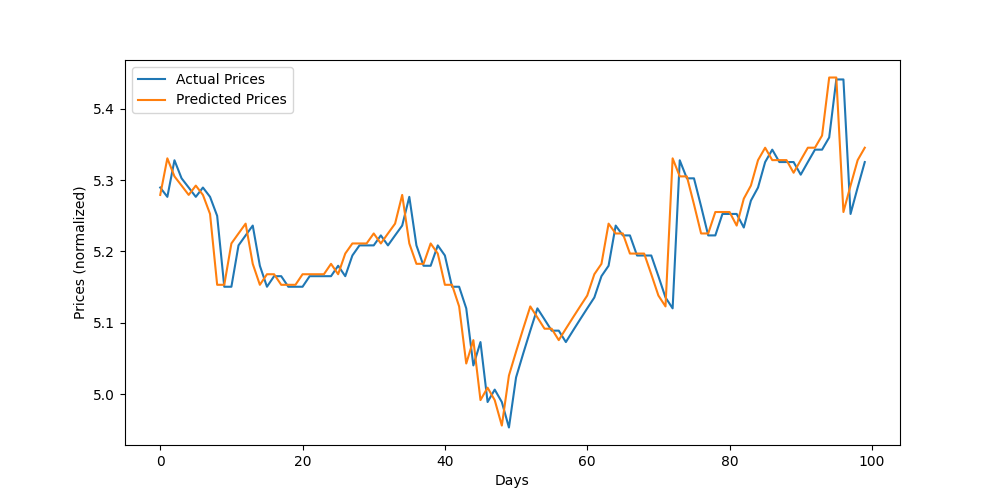
\includegraphics[width=1\textwidth]{./assets/Chapter_4/DMD_LSTM_crossval/100days/AC.png}
    \caption{Actual vs Predicted Prices on AC for 100 days}
    \label{fig:crossval100_AC}
\end{figure}
\FloatBarrier
    
% ALI
\begin{figure}[ht]
    \centering
    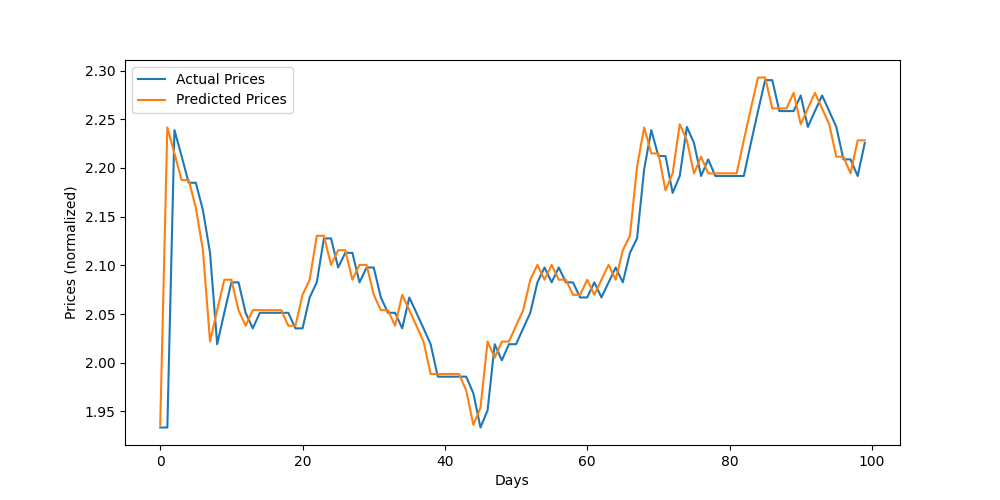
\includegraphics[width=1\textwidth]{./assets/Chapter_4/DMD_LSTM_crossval/100days/ALI.png}
    \caption{Actual vs Predicted Prices for ALI over 100 days}
    \label{fig:crossval100_ALI}
\end{figure}
\FloatBarrier

% AP
\begin{figure}[ht]
    \centering
    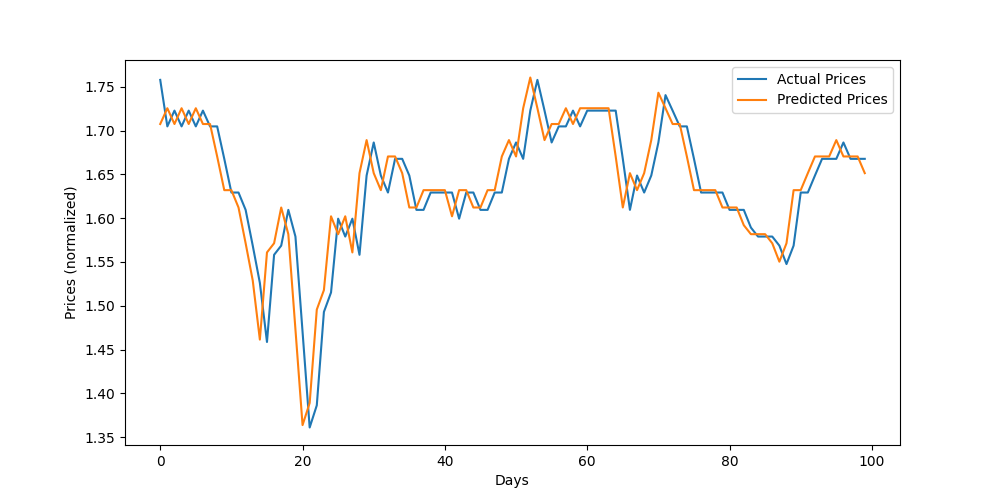
\includegraphics[width=1\textwidth]{./assets/Chapter_4/DMD_LSTM_crossval/100days/AP.png}
    \caption{Actual vs Predicted Prices for AP over 100 days}
    \label{fig:crossval100_AP}
\end{figure}
\FloatBarrier

% BDO
\begin{figure}[ht]
    \centering
    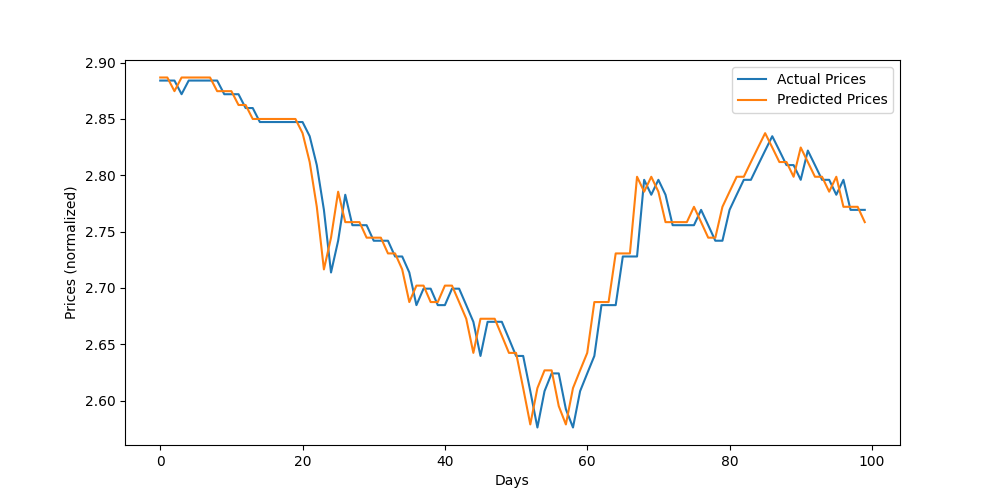
\includegraphics[width=1\textwidth]{./assets/Chapter_4/DMD_LSTM_crossval/100days/BDO.png}
    \caption{Actual vs Predicted Prices for BDO over 100 days}
    \label{fig:crossval100_BDO}
\end{figure}
\FloatBarrier

% BLOOM
\begin{figure}[ht]
    \centering
    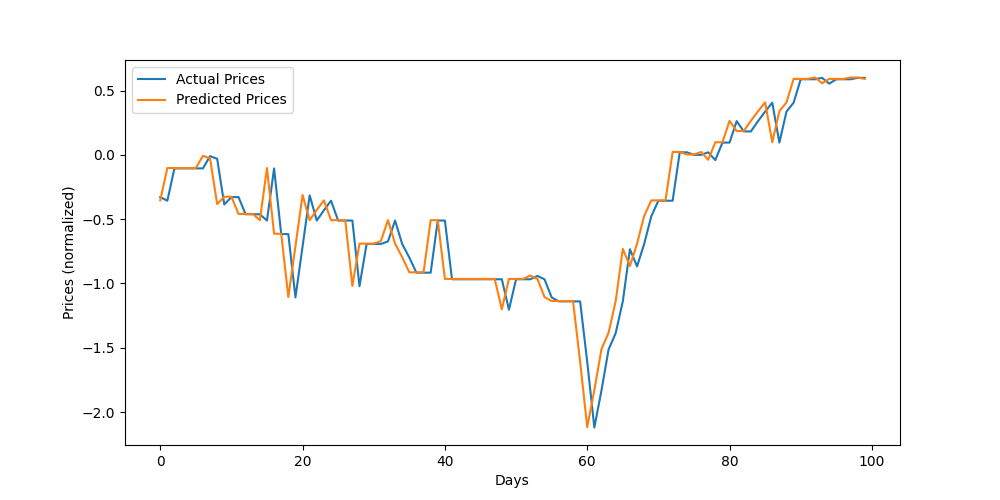
\includegraphics[width=1\textwidth]{./assets/Chapter_4/DMD_LSTM_crossval/100days/BLOOM.png}
    \caption{Actual vs Predicted Prices for BLOOM over 100 days}
    \label{fig:crossval100_BLOOM}
\end{figure}
\FloatBarrier

% FGEN
\begin{figure}[ht]
    \centering
    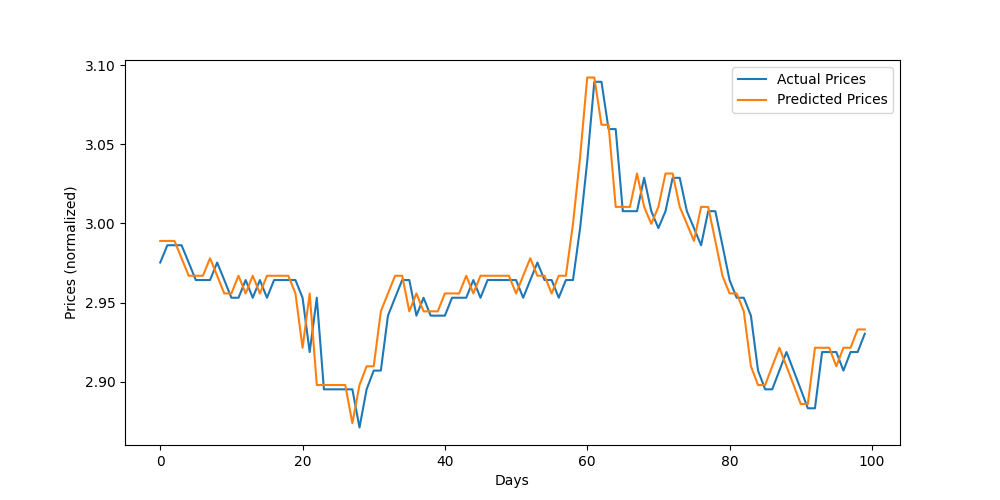
\includegraphics[width=1\textwidth]{./assets/Chapter_4/DMD_LSTM_crossval/100days/FGEN.png}
    \caption{Actual vs Predicted Prices for FGEN over 100 days}
    \label{fig:crossval100_FGEN}
\end{figure}
\FloatBarrier

% GLO
\begin{figure}[ht]
    \centering
    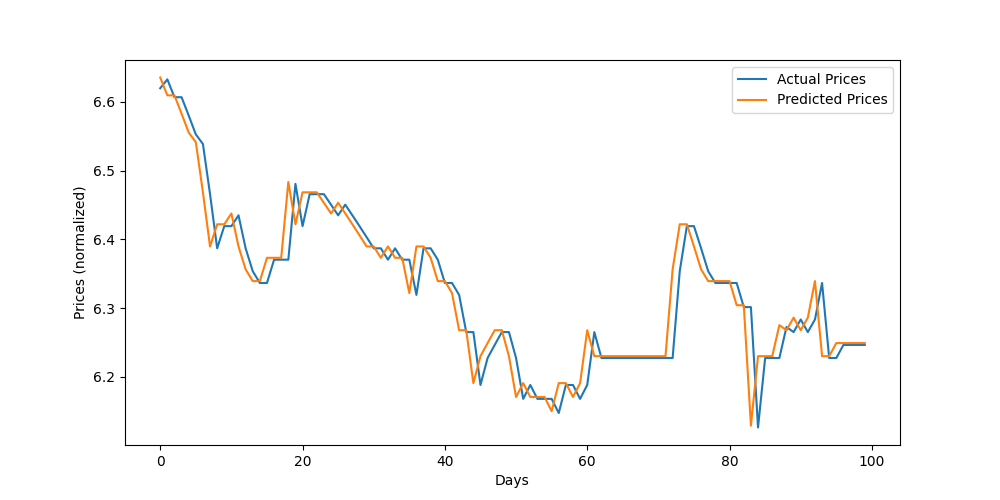
\includegraphics[width=1\textwidth]{./assets/Chapter_4/DMD_LSTM_crossval/100days/GLO.png}
    \caption{Actual vs Predicted Prices for GLO over 100 days}
    \label{fig:crossval100_GLO}
\end{figure}
\FloatBarrier

% ICT
\begin{figure}[ht]
    \centering
    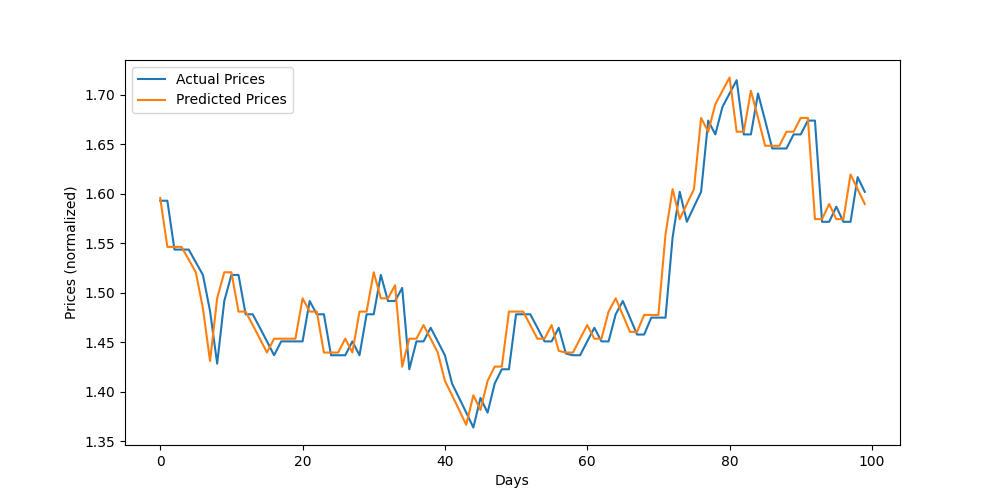
\includegraphics[width=1\textwidth]{./assets/Chapter_4/DMD_LSTM_crossval/100days/ICT.png}
    \caption{Actual vs Predicted Prices for ICT over 100 days}
    \label{fig:crossval100_ICT}
\end{figure}
\FloatBarrier

% JGS
\begin{figure}[ht]
    \centering
    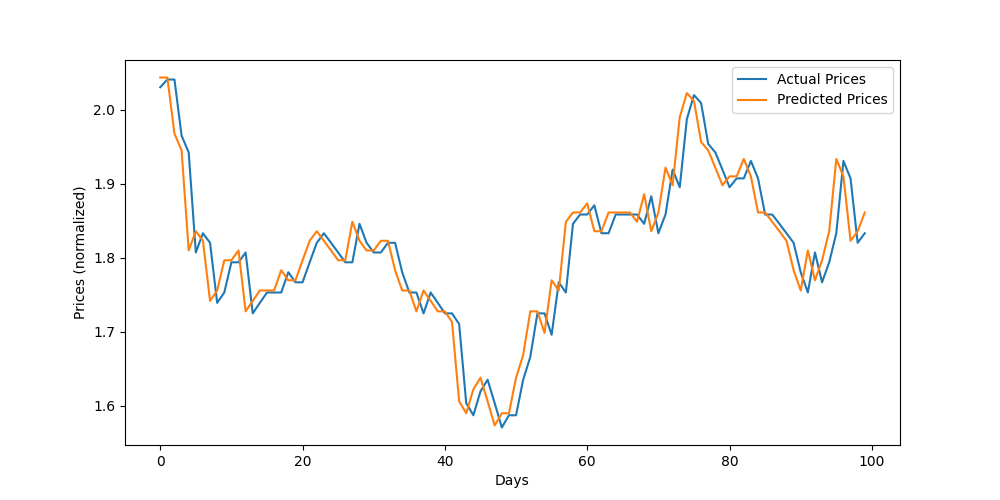
\includegraphics[width=1\textwidth]{./assets/Chapter_4/DMD_LSTM_crossval/100days/JGS.png}
    \caption{Actual vs Predicted Prices on JGS for 100 days}
    \label{fig:crossval100_JGS}
\end{figure}
\FloatBarrier
    
% LTG
\begin{figure}[ht]
    \centering
    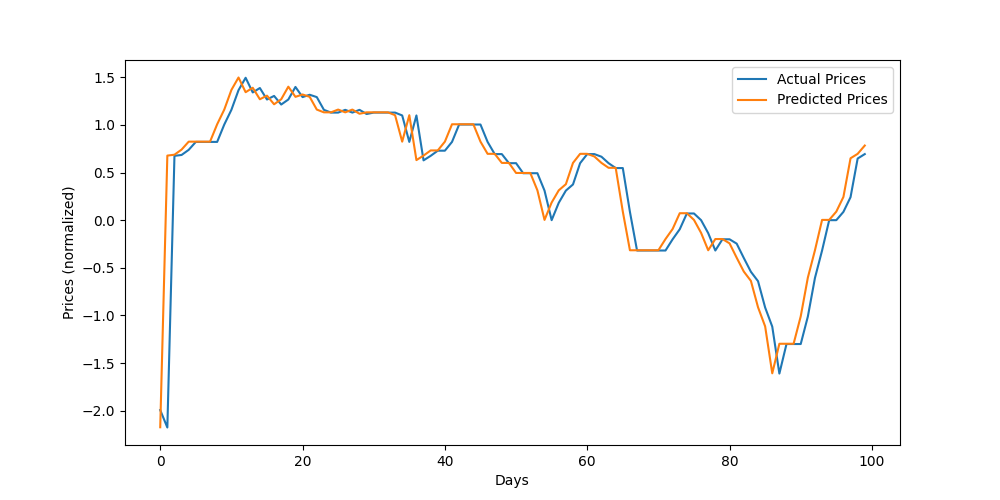
\includegraphics[width=1\textwidth]{./assets/Chapter_4/DMD_LSTM_crossval/100days/LTG.png}
    \caption{Actual vs Predicted Prices on LTG for 100 days}
    \label{fig:crossval100_LTG}
\end{figure}
\FloatBarrier

% MEG
\begin{figure}[ht]
    \centering
    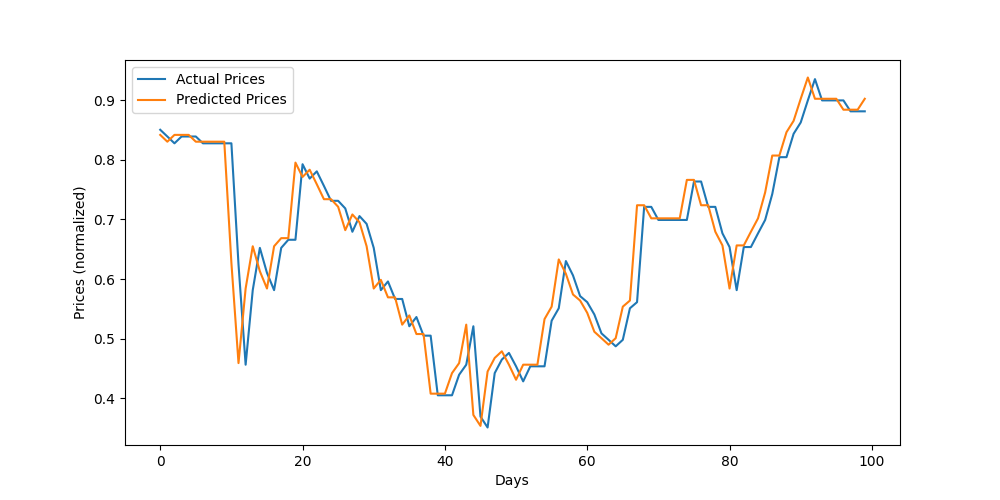
\includegraphics[width=1\textwidth]{./assets/Chapter_4/DMD_LSTM_crossval/100days/MEG.png}
    \caption{Actual vs Predicted Prices on MEG for 100 days}
    \label{fig:crossval100_MEG}
\end{figure}
\FloatBarrier

% MER
\begin{figure}[ht]
    \centering
    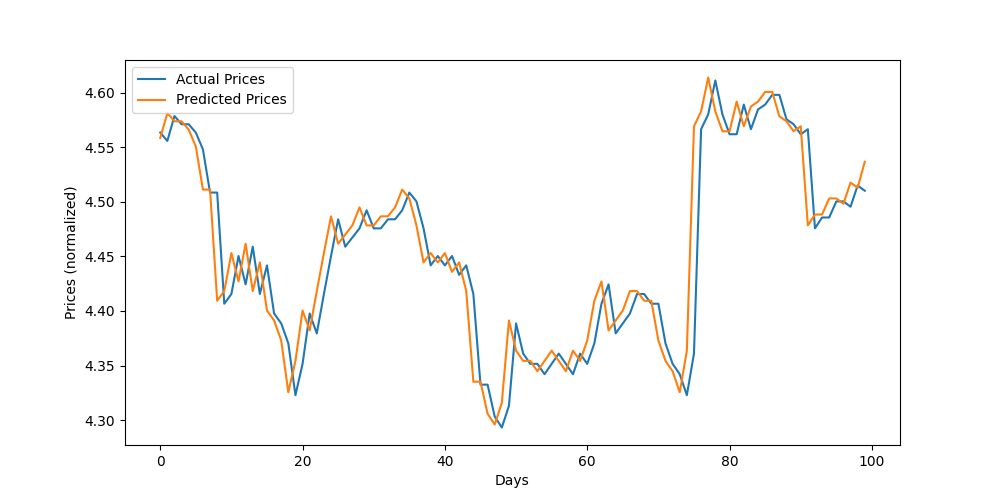
\includegraphics[width=1\textwidth]{./assets/Chapter_4/DMD_LSTM_crossval/100days/MER.png}
    \caption{Actual vs Predicted Prices on MER for 100 days}
    \label{fig:crossval100_MER}
\end{figure}
\FloatBarrier

% MPI
\begin{figure}[ht]
    \centering
    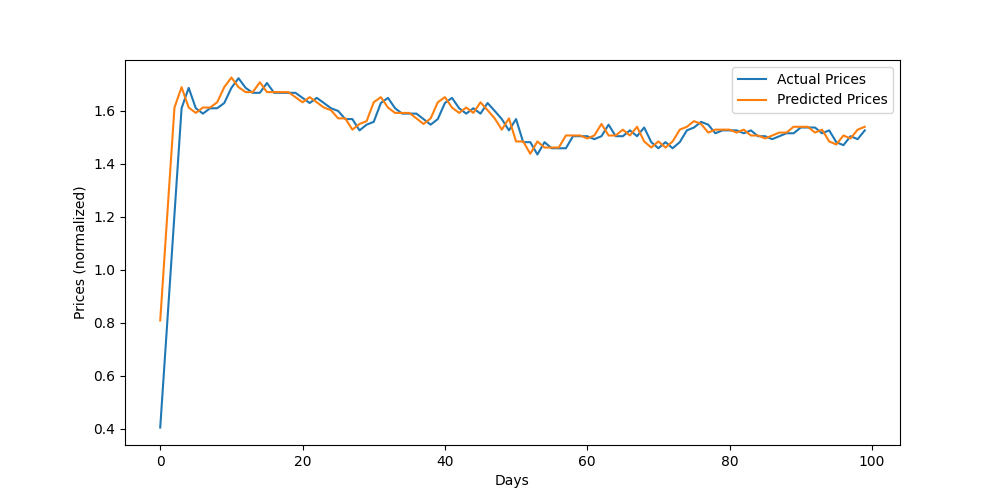
\includegraphics[width=1\textwidth]{./assets/Chapter_4/DMD_LSTM_crossval/100days/MPI.png}
    \caption{Actual vs Predicted Prices on MPI for 100 days}
    \label{fig:crossval100_MPI}
\end{figure}
\FloatBarrier

% PGOLD
\begin{figure}[ht]
    \centering
    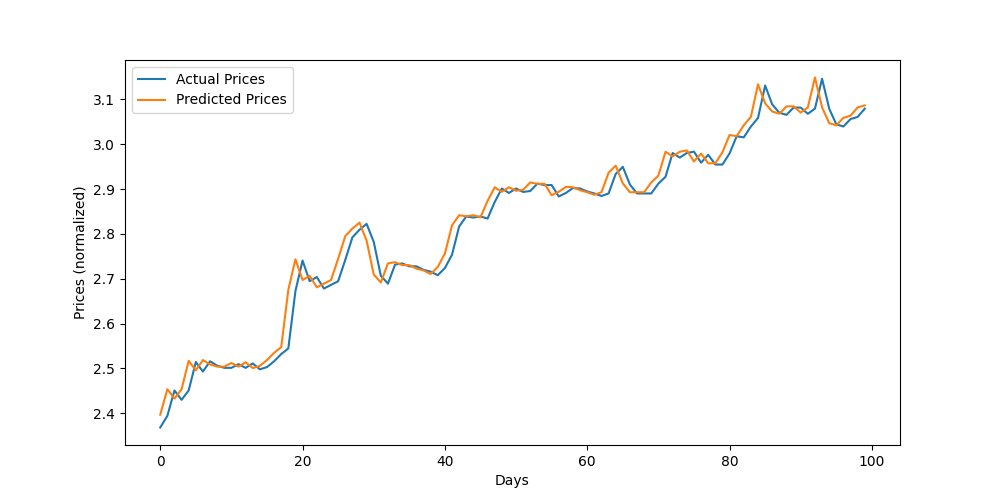
\includegraphics[width=1\textwidth]{./assets/Chapter_4/DMD_LSTM_crossval/100days/PGOLD.png}
    \caption{Actual vs Predicted Prices on PGOLD for 100 days}
    \label{fig:crossval100_PGOLD}
\end{figure}
\FloatBarrier

% PSEI
\begin{figure}[ht]
    \centering
    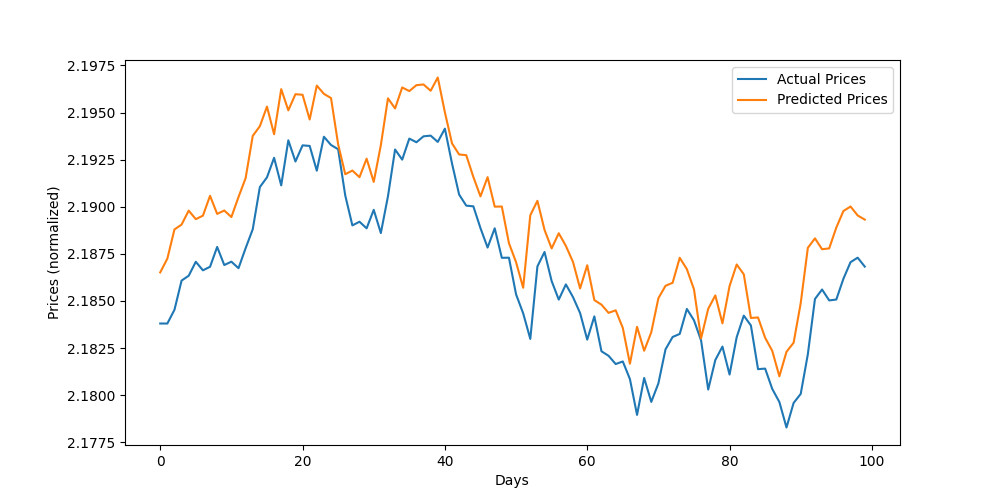
\includegraphics[width=1\textwidth]{./assets/Chapter_4/DMD_LSTM_crossval/100days/PSEI.png}
    \caption{Actual vs Predicted Prices on PSEI for 100 days}
    \label{fig:crossval100_PSEI}
\end{figure}
\FloatBarrier

% RLC
\begin{figure}[ht]
    \centering
    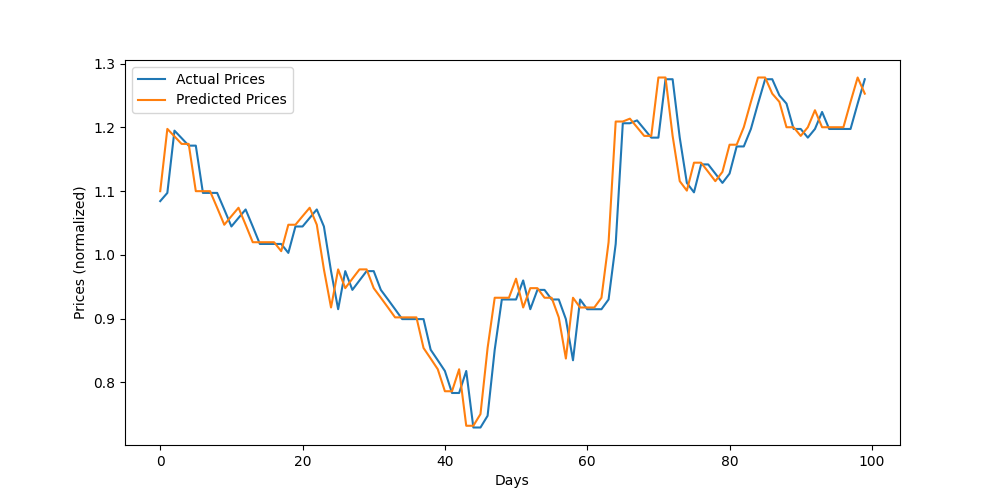
\includegraphics[width=1\textwidth]{./assets/Chapter_4/DMD_LSTM_crossval/100days/RLC.png}
    \caption{Actual vs Predicted Prices on RLC for 100 days}
    \label{fig:crossval100_RLC}
\end{figure}
\FloatBarrier

% RRHI
\begin{figure}[ht]
    \centering
    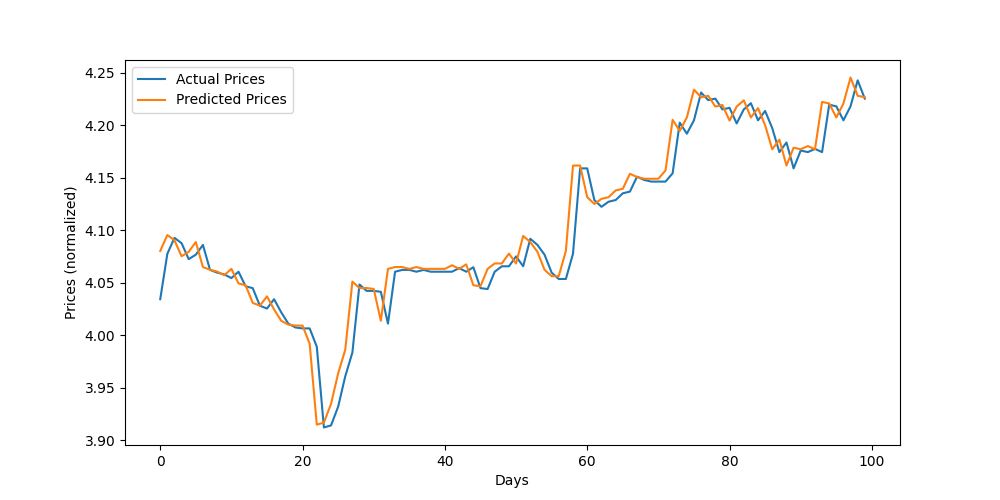
\includegraphics[width=1\textwidth]{./assets/Chapter_4/DMD_LSTM_crossval/100days/RRHI.png}
    \caption{Actual vs Predicted Prices on RRHI for 100 days}
    \label{fig:crossval100_RRHI}
\end{figure}
\FloatBarrier

% SMC
\begin{figure}[ht]
    \centering
    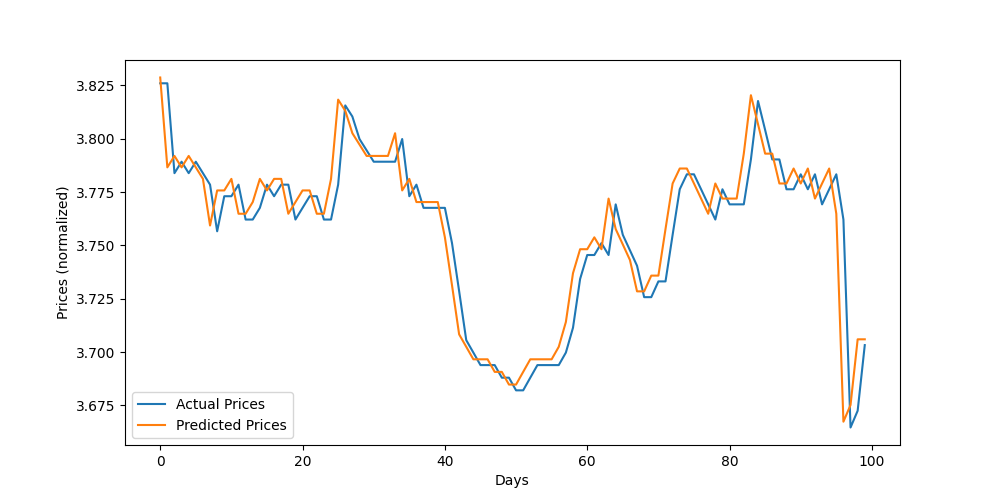
\includegraphics[width=1\textwidth]{./assets/Chapter_4/DMD_LSTM_crossval/100days/SMC.png}
    \caption{Actual vs Predicted Prices on SMC for 100 days}
    \label{fig:crossval100_SMC}
\end{figure}
\FloatBarrier

% TEL
\begin{figure}[ht]
    \centering
    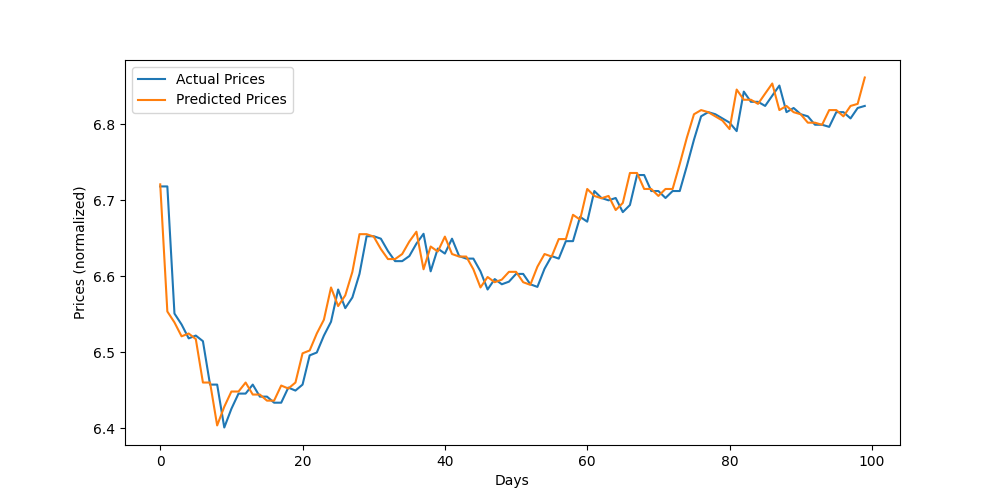
\includegraphics[width=1\textwidth]{./assets/Chapter_4/DMD_LSTM_crossval/100days/TEL.png}
    \caption{Actual vs Predicted Prices on TEL for 100 days}
    \label{fig:crossval100_TEL}
\end{figure}
\FloatBarrier

% URC
\begin{figure}[ht]
    \centering
    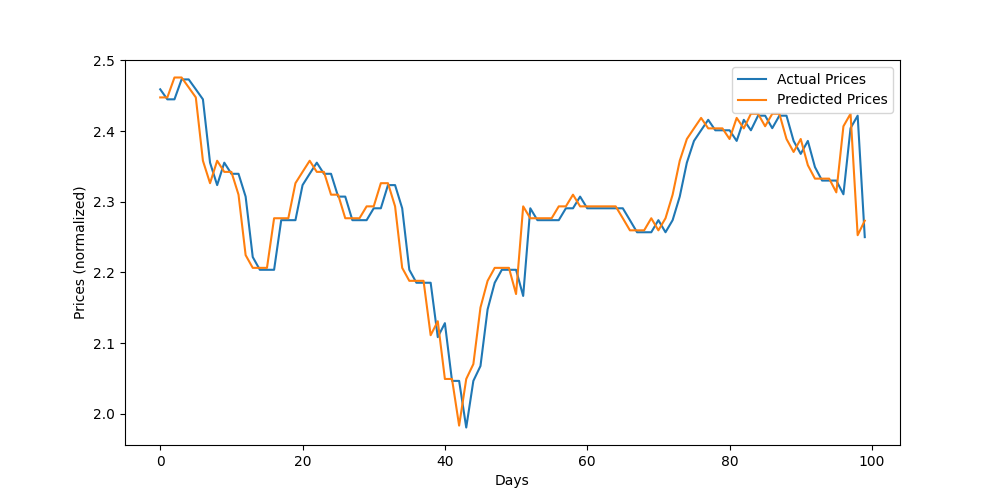
\includegraphics[width=1\textwidth]{./assets/Chapter_4/DMD_LSTM_crossval/100days/URC.png}
    \caption{Actual vs Predicted Prices on URC for 100 days}
    \label{fig:crossval100_URC}
\end{figure}
\FloatBarrier}
The figures above show that the predicted prices follow the actual 
price trend. In addition, the discrepancy between predicted and 
actual prices is relatively small, as evidenced by the error metrics 
scores shown in Table \ref{tab:dmd-lstm_cross}.
\\

However, the MAPE scores for BLOOM, ICT, JGS, LTG, and MEG range from 
ten billion to hundred billion. This outlier in the data is, 
fortunately, just the result of the applied logarithmic normalization, 
where some of the data in the datasets of the aforementioned stocks 
are in the negative range, that influence the calculation of the 
MAPE scores using the scikit-learn library. Because this library 
handles the calculation of the MAPE scores, there is no way to fix 
this bug. Moreover, if we take a look at the 
graphs of the 100 days prediction versus the actual for the
aforementioned stocks in Figures
\ref{fig:crossval100_BLOOM},
\ref{fig:crossval100_ICT},
\ref{fig:crossval100_JGS},
\ref{fig:crossval100_LTG}, and
\ref{fig:crossval100_MEG}, respectively, it can still be observed
that the model performs well on these stocks.
\\

Not to mention that the other error metrics used show the same 
performance levels across the different stocks when the DMD-LSTM
model is utilized. Meanwhile when the data normalization is removed, 
the MAPE scores for BLOOM, ICT, JGS, LTG, and MEG become 0.068108, 
0.037207, 0.039754, 0.057332, and 0.044411 units, respectively.
\\

The successive predictions for the following day and up to ten days 
were tested using the price data from PSEI in order to make the 
system's predictions more useful for actual utilization.
Table \ref{tab:dmd-lstm_succpreds} shows 
the MAPE scores for the successive predictions of the DMD-LSTM
for each days.
% tab:dmd-lstm_succpreds
\begin{longtable}[c]{ccc}
    \caption{DMD-LSTM Successive Predictions}
    \label{tab:dmd-lstm_succpreds}\\
    \hline
    \textbf{\begin{tabular}[c]{@{}c@{}}Successive \\ Days Predicted\end{tabular}} & \textbf{\begin{tabular}[c]{@{}c@{}}Actual and Predicted \\ Data Ratio\end{tabular}} & \textbf{\begin{tabular}[c]{@{}c@{}}MAPE \\ Score\end{tabular}} \\ \hline
    \endfirsthead
    %
    \multicolumn{3}{c}%
    {{\bfseries Table \thetable\ continued from previous page}} \\
    \hline
    \textbf{\begin{tabular}[c]{@{}c@{}}Successive \\ Days Predicted\end{tabular}} & \textbf{\begin{tabular}[c]{@{}c@{}}Actual and Predicted \\ Data Ratio\end{tabular}} & \textbf{\begin{tabular}[c]{@{}c@{}}MAPE \\ Score\end{tabular}} \\ \hline
    \endhead
    %
    \hline
    \endfoot
    %
    \endlastfoot
    %
    1                                                                             & 100\%                                                                               & 0.00973                                                        \\
    2                                                                             & 80\%                                                                                & 0.13403                                                        \\
    3                                                                             & 60\%                                                                                & 0.15782                                                        \\
    4                                                                             & 40\%                                                                                & 0.15646                                                        \\
    5                                                                             & 20\%                                                                                & 0.13910                                                        \\
    6                                                                             & {\color[HTML]{FE0000} 0\%}                                                          & 0.12494                                                        \\
    7                                                                             & {\color[HTML]{FE0000} -20\%}                                                        & 0.11283                                                        \\
    8                                                                             & {\color[HTML]{FE0000} -40\%}                                                        & 0.10014                                                        \\
    9                                                                             & {\color[HTML]{FE0000} -60\%}                                                        & 0.08914                                                        \\
    10                                                                            & {\color[HTML]{FE0000} -100\%}                                                       & 0.08976                                                        \\ \hline
\end{longtable}}
From the table above it must be noted that the ratio values highlighted in red 
is to demonstrate that, despite the fact that negative ratio values shouldn't 
exist, doing so simply indicates that the data used to forecast the subsequent 
price data was overlapping by 2 to 5 times, depending on the ratio, and no 
longer used any actual data.
\\

Moreover, in the integration of the DMD-LSTM model to the alamSYS, the
5 days successive predictions was utilized. Where it is shown
from the Table \ref{tab:dmd-lstm_succpreds} that it still performs
well, even if the actual and predicted data ratio is only at 20\%.
This is also to limit the effect of stock market volatility that
might affect the accuracy of the successive predictions of the model.
\\

However, it can also be observed that the MAPE scores for
successive days with zero to negative actual and predicted data
ratio outperforms the MAPE scores from successive days 2 to 5
as illustrated in Figure \ref{fig:MAPE_successive}, shown below.
\hfill \\

\begin{figure}[ht]
    \centering
    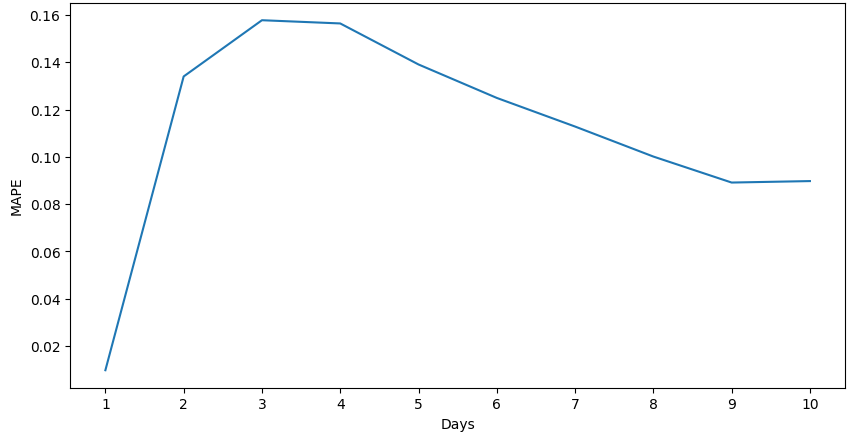
\includegraphics[width=1\textwidth]{./assets/Chapter_4/MAPE_successive.png}
    \caption{MAPE Scores for 1 to 10 (Days) Successive Predictions}
    \label{fig:MAPE_successive}
\end{figure}
\FloatBarrier

Yet, since doing so might result in a poor generalization of data, 
they were not chosen to be the maximum consecutive days of predictions 
to be integrated in the alamSYS. As a matter of fact, it could be 
argued that these data's MAPE scores are overfitted, rendering them 
unreliable. On the contrary, it might also imply that the model 
maintains its accuracy for a longer time, even if the majority of 
the data used are those produced by the model itself. This could be 
a good thing, and may be attributed to the use of the dynamic modes,
as first suggested in the study of \citeA{Mann2015}.
In light of these considerations, additional testing is required to 
establish which of the two claims is true.

Overall, the results from the model training, evaluation, and cross-validation
shows that the DMD-LSTM model developed in this special problem performs
on par with the other studies that utilizes dynamic modes, as mentioned in 
Chapter \ref{chap:lit_review} of this paper.